\documentclass[12pt]{article}

% Basic math support
\usepackage[utf8]{inputenc}
\usepackage{amsmath, amsfonts, amssymb}

% Page setup
\usepackage{geometry}
\geometry{margin=1in}
\usepackage{float}
\usepackage{hyperref}

% for images
\usepackage{graphicx}

% Metadata
\title{MTH/CSC 4150 \\ Fall 2025 \\ Draft Project Report:\\
Mathematically Modeling a Distance Runner's Race with Interpolation}
\author{Daron Baltazar, Evan Dant, Madi Price}
\date{Friday, December 5th}

\begin{document}

\maketitle

\section{Introduction}

Researchers have developed many ways to predict running performance and maximize
athletic potential \cite{Dash}. Traditional regression models are frequently used
for this purpose \cite{MillettMelanson}, but numerical interpolation methods can
also reveal structure in race pacing data. Online tools already combine interpolation
and extrapolation to estimate finish times from partial race results, as seen in
various running calculators.\footnote{For example:
\url{https://wismuth.com/running/calculator.html}.}

In this project, we model a runner's cumulative race distance as a function of
time, denoted by $s(t)$. From this interpolated position function, we approximate
the instantaneous velocity $v(t)$ and acceleration $a(t)$. We compare three
interpolation approaches studied in class:

\begin{itemize}
  \item a Newton interpolating polynomial,
  \item a natural cubic spline,
  \item a clamped cubic spline.
\end{itemize}

We examine how the choice of interpolant and the boundary conditions affect the
estimated velocity and acceleration curves and how well each method captures
realistic pacing patterns over the course of a marathon.

\section{Theoretical Background}

\subsection{Polynomial Interpolation}

Suppose there are $n+1$ data points $(t_i, s_i)$ with distinct time values
$t_0 < t_1 < \dots < t_n$. An interpolating polynomial $p_n(t)$ of degree at most $n$
satisfies
\begin{equation}
  p_n(t_i) = s_i, \qquad i = 0,1,\dots,n.
  \label{eq:interp_condition}
\end{equation}
There exists a unique polynomial of degree at most $n$ that satisfies
the interpolation conditions in equation~(\ref{eq:interp_condition}).

In the Lagrange form,
\begin{equation}
  p_n(t) = \sum_{i=0}^{n} s_i L_i(t),
  \label{eq:lagrange_poly}
\end{equation}
where the Lagrange basis polynomials are
\begin{equation}
  L_i(t) =
  \prod_{\substack{j=0 \\ j \neq i}}^{n}
  \frac{t - t_j}{t_i - t_j},
  \qquad i = 0,1,\dots,n.
  \label{eq:lagrange_basis}
\end{equation}
This basis is interpolatory, since $L_i(t_j) = \delta_{ij}$.

In Newton's form, an alternative basis is used:
\begin{equation}
  p_n(t) =
  a_0 + a_1 (t - t_0) + a_2 (t - t_0)(t - t_1) + \dots +
  a_n \prod_{k=0}^{n-1} (t - t_k),
  \label{eq:newton_poly}
\end{equation}
where the coefficients $a_i$ are computed from divided differences.
Newton's form is more convenient for computation and for updating the
polynomial when additional data points are added.

\subsection{Interpolation Error}

Let $f(t)$ be a sufficiently smooth function and let $p_n(t)$ be the
degree-$n$ interpolating polynomial constructed from $n+1$ distinct
nodes $t_0,\dots,t_n$. The interpolation error can be written as
\begin{equation}
  f(t) - p_n(t) =
  \frac{f^{(n+1)}(c)}{(n+1)!}\,
  \prod_{i=0}^{n} (t - t_i),
  \label{eq:interp_error}
\end{equation}
for some $c$ in the interval containing the nodes and the point $t$.
This formula shows that the error depends on both the spacing of the
nodes and the $(n+1)$st derivative of $f(t)$. When the nodes are equally
spaced and $n$ is large, the product term can lead to large oscillations
near the ends of the interval (Runge's phenomenon).

\subsection{Cubic Splines}

To reduce the oscillations associated with high-degree polynomials, we
use cubic splines. Given $n+1$ knots $t_0<t_1<\dots< t_n$ and function
values $s_i = f(t_i)$, a cubic spline $S(t)$ is a piecewise cubic
polynomial of the form
\begin{equation}
  S(t) =
  \begin{cases}
    S_0(t), & t \in [t_0,t_1], \\
    S_1(t), & t \in [t_1,t_2], \\
    \vdots \\
    S_{n-1}(t), & t \in [t_{n-1},t_n],
  \end{cases}
\end{equation}
where each piece has the form
\begin{equation}
  S_i(t) = a_i + b_i (t - t_i) + c_i (t - t_i)^2 + d_i (t - t_i)^3.
  \label{eq:spline_piece}
\end{equation}
The spline is constructed so that
\begin{enumerate}
  \item $S(t_i) = s_i$ and $S(t_{i+1}) = s_{i+1}$ for $i = 0,\dots,n-1$
        (interpolation),
  \item $S(t)$ is continuously differentiable, so $S'(t)$ is continuous at
        each interior knot $t_1,\dots,t_{n-1}$,
  \item $S''(t)$ is continuous at each interior knot.
\end{enumerate}
These conditions yield $4n-2$ equations. Two additional conditions are
needed at the endpoints.

In a \emph{natural} cubic spline, the second derivative is set to zero
at both ends:
\begin{equation}
  S''(t_0) = 0, \qquad S''(t_n) = 0.
  \label{eq:natural_bc}
\end{equation}

In a \emph{clamped} cubic spline, the slopes at the endpoints are
specified directly:
\begin{equation}
  S'(t_0) = v_0, \qquad S'(t_n) = v_n,
  \label{eq:clamped_bc}
\end{equation}
where $v_0$ and $v_n$ are prescribed velocities. In our setting these
slopes are estimated from one-sided finite differences at the beginning
and end of the marathon. This allows the model to encode physically
meaningful information about the runner's starting and finishing pace.

Solving the resulting linear systems produces the coefficients
$a_i,b_i,c_i,d_i$ for all subintervals.

\subsection{Numerical Differentiation}

Once a smooth interpolating function $S(t)$ is available, the velocity
and acceleration of the runner are given by
\begin{equation}
  v(t) = S'(t), \qquad a(t) = S''(t).
  \label{eq:vel_acc}
\end{equation}
For spline models, derivatives can be computed analytically by
differentiating the cubic expressions in equation~(\ref{eq:spline_piece}),
or numerically using finite difference stencils.

For comparison, numerical differentiation formulas can also be derived
directly from discrete data or from an interpolant evaluated on a fine
time grid. For example, the centered difference approximation for the
first derivative at an interior node is
\begin{equation}
  f'(t_i) \approx
  \frac{f(t_{i+1}) - f(t_{i-1})}{2h},
  \label{eq:centered_diff}
\end{equation}
where $h = t_{i+1} - t_i$ is the time step. This stencil is second
order accurate in $h$.

\section{Data and Preprocessing}

The data for this project consist of split times and cumulative
distances from a single distance runner's race. Let $t_i$ denote the elapsed time at the
$i$th checkpoint and let $s_i$ denote the cumulative distance at this
time.

We work with data from the New York City Marathon, taken from the New
York Road Runners results website. The runner is a recreational female
participant (our professor's sister-in-law), which provides a realistic,
non-elite pacing profile for a full marathon. The splits include a mix
of mile and kilometer markers, which are converted to consistent units.

\begin{figure}[H]
  \centering
  \textbf{NYC Marathon Split Times}\\[0.5em]
  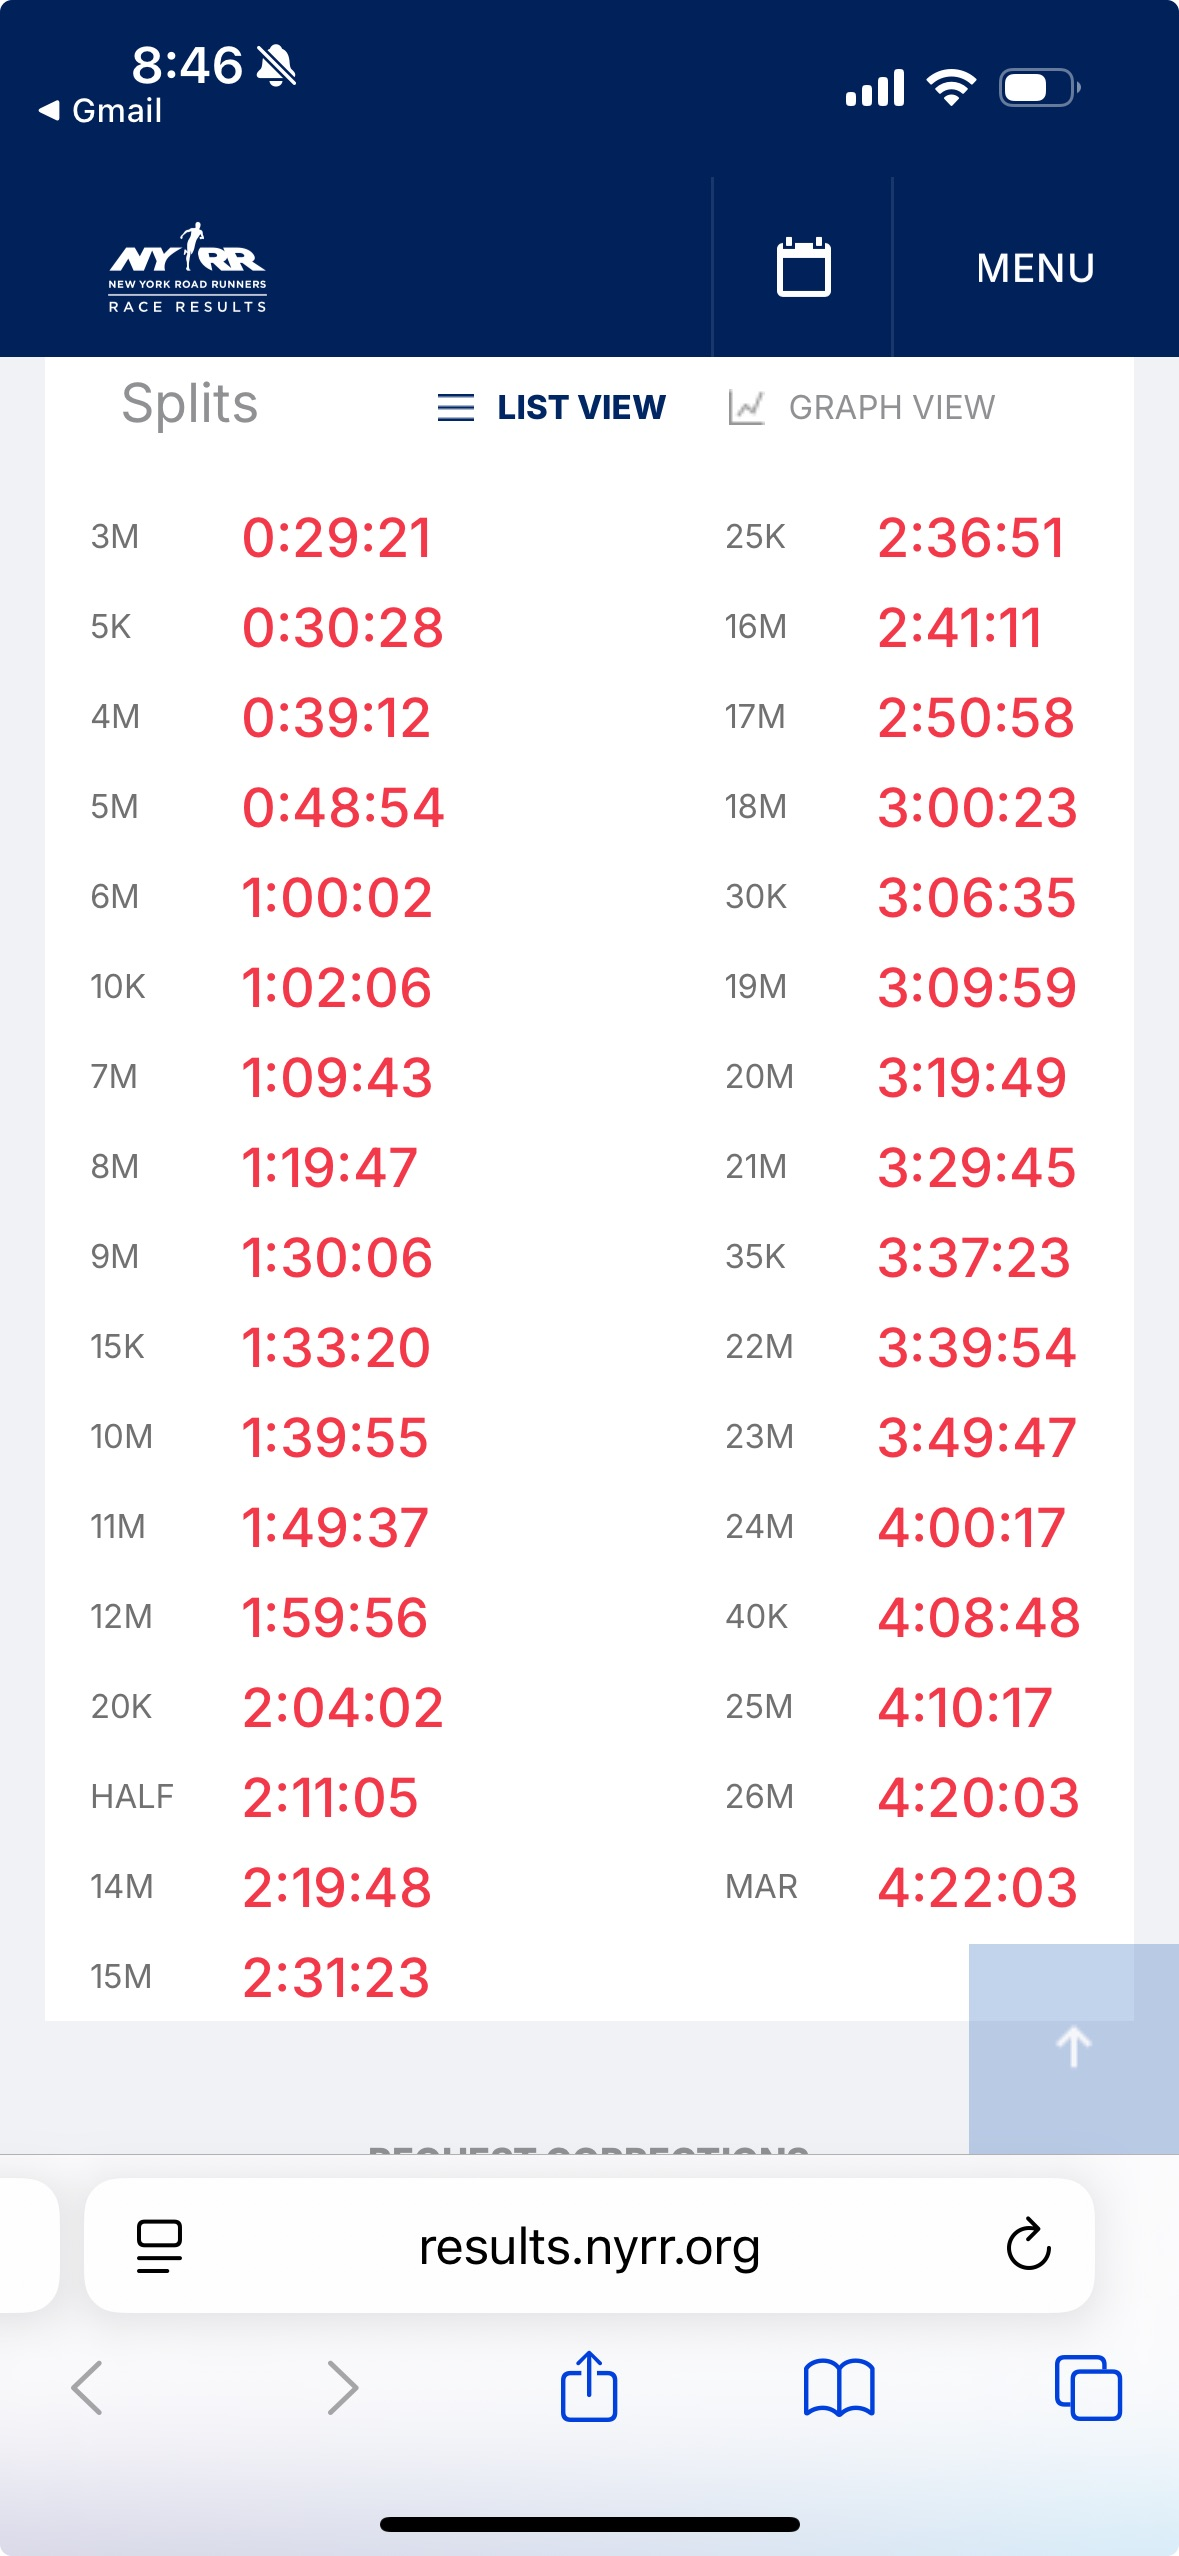
\includegraphics[width=0.85\linewidth]{NYRR_splits.png}
  \caption{NYC Marathon split times for a recreational female runner
  (NYRR results page).}
  \label{fig:splits}
\end{figure}

We perform the following preprocessing steps:
\begin{enumerate}
\item Convert all distances to meters and all times to seconds, using the
      standard conversions $1\text{ mile} \approx 1609\text{ m}$ and
      $1\text{ km} = 1000\text{ m}$.
\item Shift the time axis so that $t_0 = 0$ at the race start.
\item Check for and remove any obvious measurement errors, such as
      negative time differences between consecutive splits. (The
      provided dataset did not require any corrections.)
\end{enumerate}
The resulting data $\{(t_i, s_i)\}_{i=0}^n$ serve as the input to
all interpolation methods. These same processed values appear in the
MATLAB driver script used to generate our figures.

\section{Numerical Methods and Implementation}

\subsection{Interpolation Models}

We implement and compare the following models in MATLAB.

\begin{enumerate}
\item \textbf{Newton polynomial interpolation.}
      We construct the interpolating polynomial in Newton form using
      a custom function \texttt{newtondd.m}, which computes the divided
      differences and evaluates the resulting polynomial by nested
      multiplication with base points. This approach provides a useful
      baseline but is expected to be sensitive to node spacing and prone
      to endpoint oscillations.

\item \textbf{Natural cubic spline.}
      We build a natural cubic spline using a routine
      \texttt{splinecoeff\_natural.m}, following the structure of
      Sauer's Program 3.5. A companion function \texttt{eval\_spline\_nat.m}
      evaluates $S(t)$, $S'(t)$, and $S''(t)$ analytically on a fine
      time grid.

\item \textbf{Clamped cubic spline.}
      We construct a clamped spline with endpoint slope conditions
      given by equation~(\ref{eq:clamped_bc}). The slopes $v_0$ and
      $v_n$ are estimated using one-sided finite differences at the
      start and end of the race:
      \[
        v_0 \approx \frac{s_1 - s_0}{t_1 - t_0}, \qquad
        v_n \approx \frac{s_n - s_{n-1}}{t_n - t_{n-1}}.
      \]
      The coefficients are computed with \texttt{splinecoeff\_clamped.m}
      and evaluated with the same \texttt{eval\_spline\_nat.m} routine.
\end{enumerate}

\subsection{Velocity and Acceleration}

For the spline models, we compute the velocity and acceleration by
differentiating the cubic spline pieces analytically. For a single
interval,
\[
  S_i(t) = a_i + b_i (t - t_i) + c_i (t - t_i)^2 + d_i (t - t_i)^3,
\]
the first and second derivatives are
\begin{equation}
  S_i'(t) = b_i + 2 c_i (t - t_i) + 3 d_i (t - t_i)^2,
  \label{eq:spline_first_deriv}
\end{equation}
\begin{equation}
  S_i''(t) = 2 c_i + 6 d_i (t - t_i).
  \label{eq:spline_second_deriv}
\end{equation}
Evaluating equations~(\ref{eq:spline_first_deriv}) and
(\ref{eq:spline_second_deriv}) on a fine time grid yields approximate
velocity and acceleration profiles for the runner.

For the Newton polynomial model, we first evaluate $p_n(t)$ on an
equally spaced time mesh. We then apply the centered-difference
stencil~(\ref{eq:centered_diff}) to approximate $v(t)$ and apply the
same stencil again to approximate $a(t)$. This provides a consistent
finite-difference framework for comparing polynomial-based and
spline-based derivatives.

\subsection{Accuracy Checks}

We validate the interpolants in one main way:
\begin{enumerate}
\item \textbf{Checkpoint consistency.} For each method, we verify that
      the interpolant reproduces the input distances at the original
      split times, i.e., $S(t_i) \approx s_i$. Because all three methods
      are true interpolants, this consistency check is passed exactly up
      to numerical roundoff error.
\end{enumerate}

\section{Results}

\subsection{Position vs.\ Time}

Figure~\ref{fig:position} displays cumulative distance versus elapsed
time for the Newton interpolating polynomial, the natural cubic spline,
the clamped cubic spline, and the original split data. All three
interpolation methods pass exactly through each data point, as required
by construction, and they are nearly indistinguishable over the majority
of the race.

Small differences among the interpolants appear primarily near the
endpoints of the interval. The Newton polynomial shows a slightly
sharper curvature near the final splits compared to both spline models,
which is consistent with the oscillatory behavior associated with
high-degree polynomial interpolation near boundaries. The natural and
clamped splines remain visually smoother at the ends of the race, with
the clamped spline exhibiting the most uniform curvature due to its
imposed endpoint slope conditions.

Because the underlying split data are approximately linear for this
runner, the position plots alone do not differentiate the interpolants
strongly. The influence of the interpolation choice becomes more
pronounced after differentiation, as seen in the velocity and
acceleration results below.

\begin{figure}[H]
  \centering
  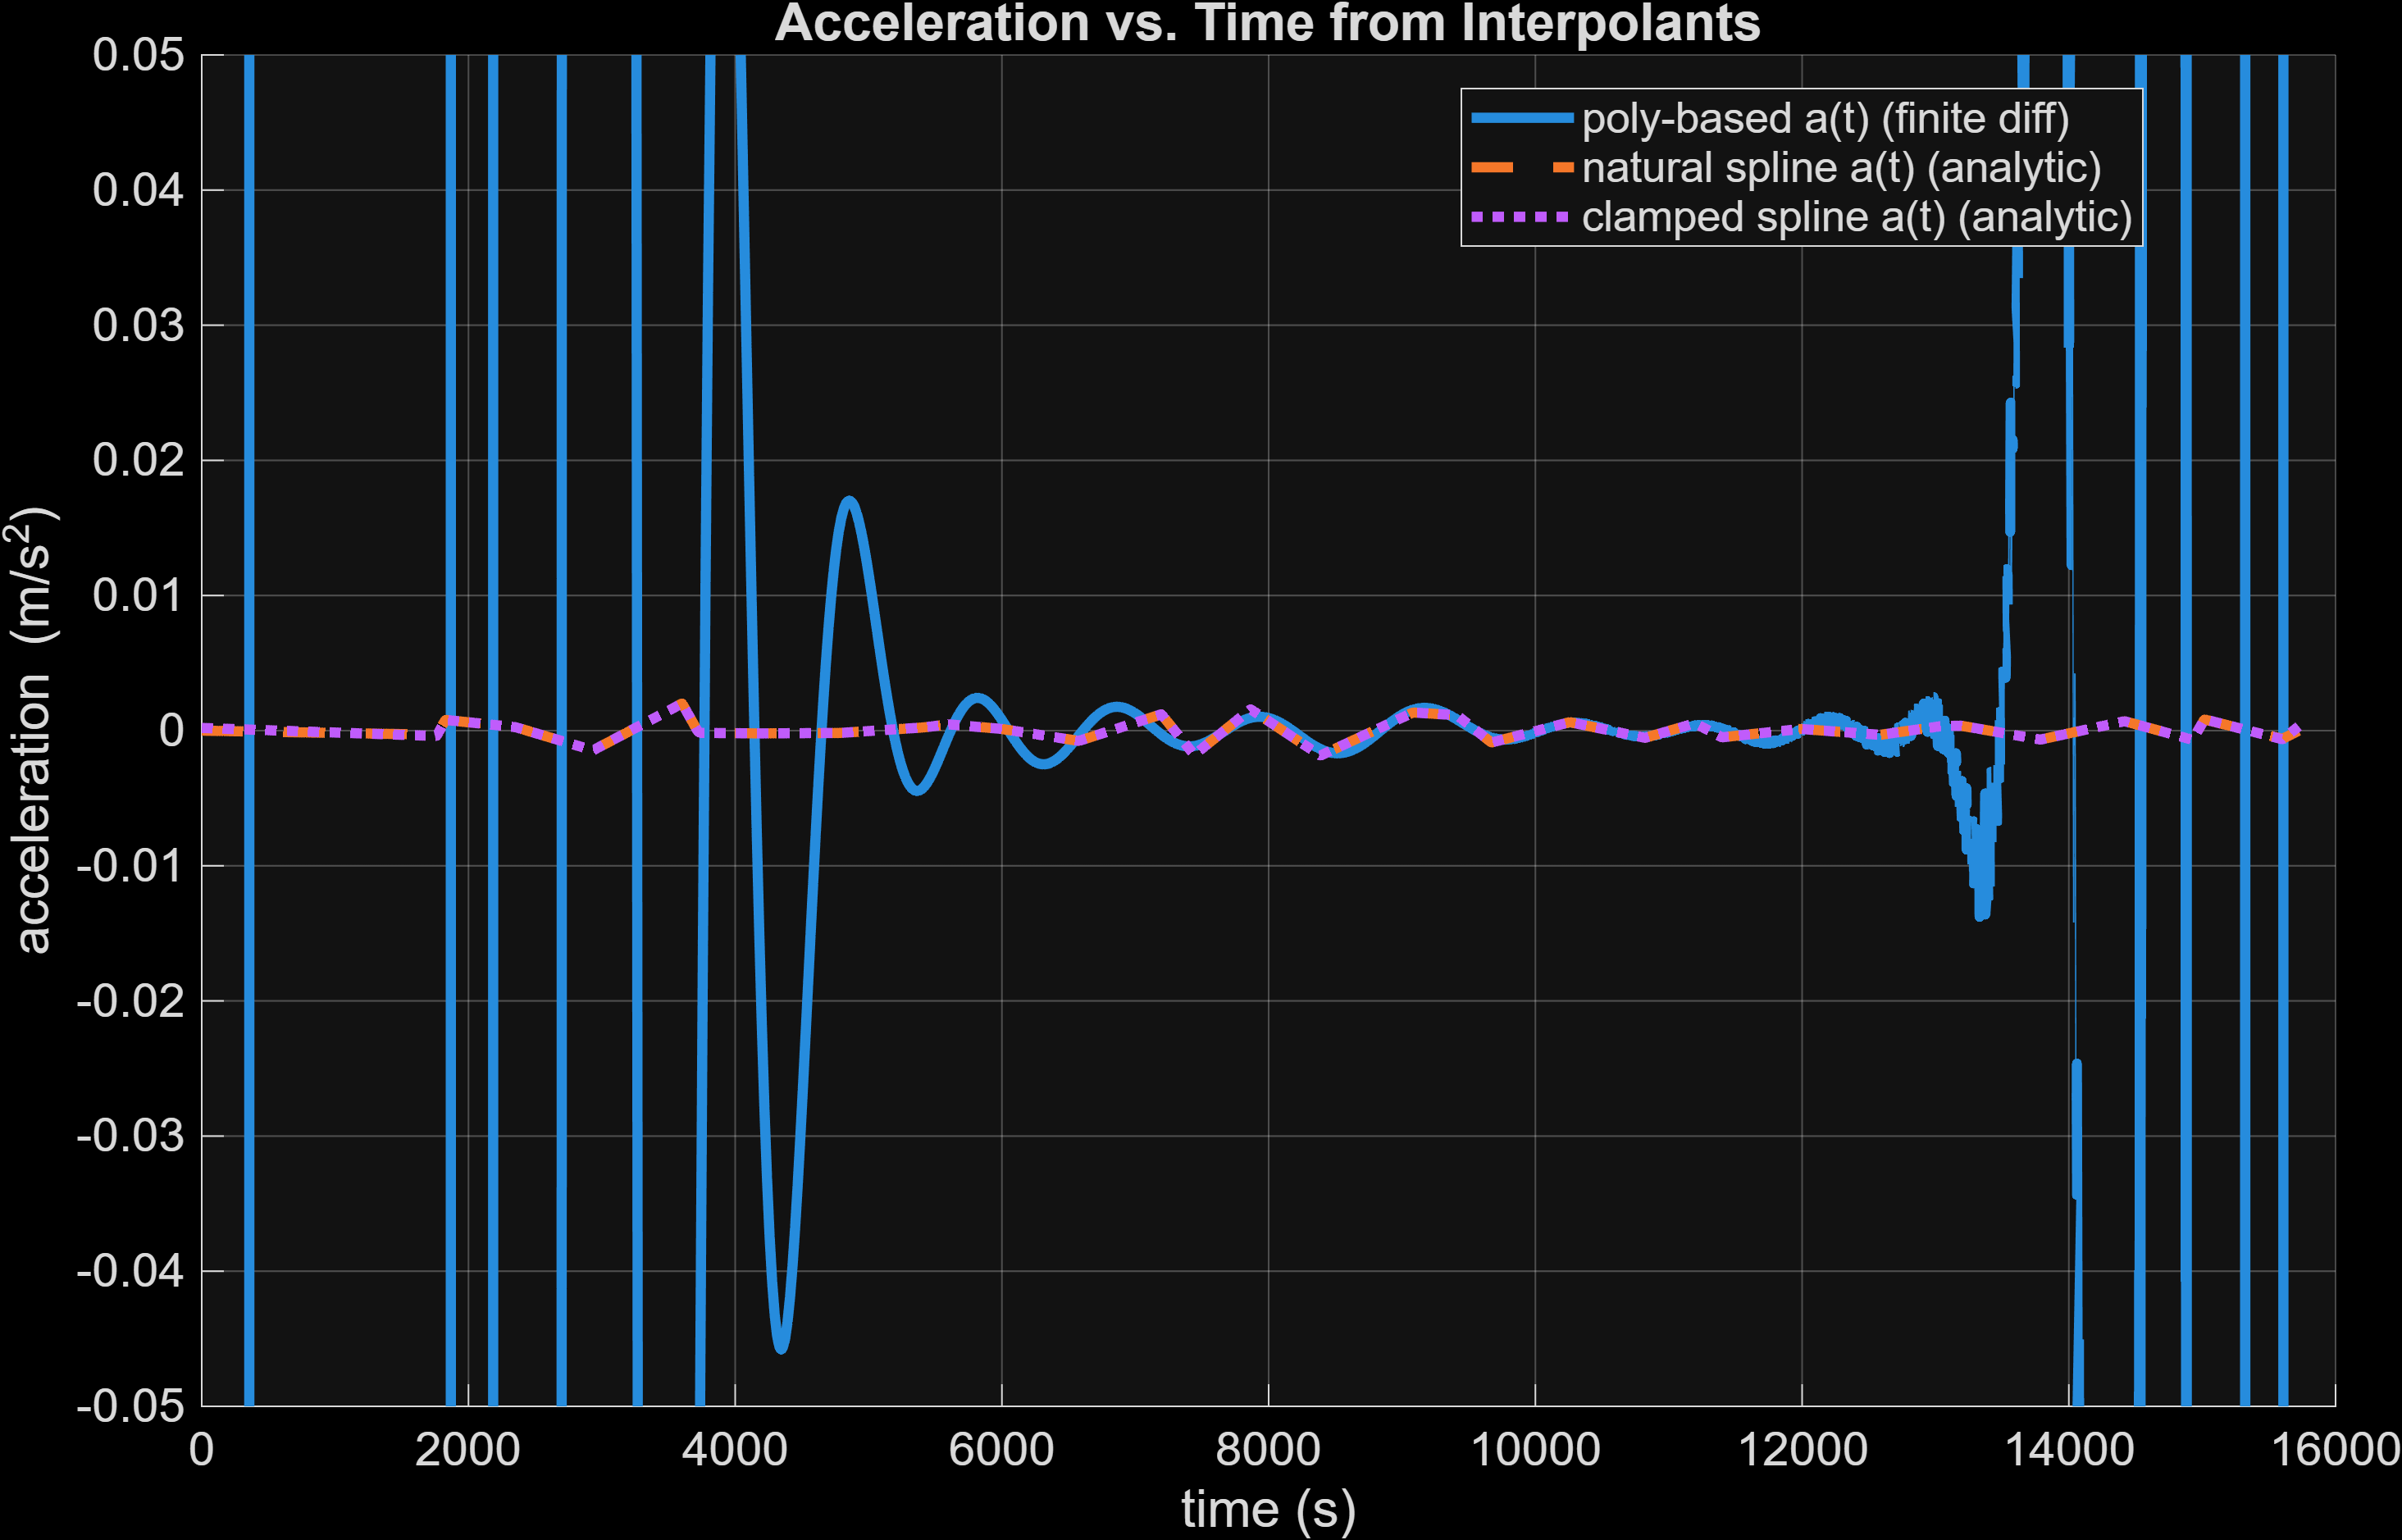
\includegraphics[width=0.85\linewidth]{PosvTime.png}
  \caption{Cumulative distance versus time for the Newton polynomial,
  natural spline, and clamped spline, together with the original split data.}
  \label{fig:position}
\end{figure}

\subsection{Velocity Profiles}

Figure~\ref{fig:velocity} displays velocity versus time computed from
each interpolation method. The velocity associated with the Newton
polynomial is computed using centered finite-difference approximations
applied to the polynomial interpolant, while the spline velocities are
computed analytically from the derivatives of the cubic piecewise
functions.

At the beginning of the race, the natural cubic spline shows a nonzero
initial velocity. This behavior is a direct consequence of the natural
spline's boundary condition in equation~(\ref{eq:natural_bc}), which
forces zero curvature at the start and prevents the model from capturing
the sharp acceleration from rest. In contrast, the polynomial-based
velocity and the clamped spline velocity both begin near zero, which is
more consistent with physical race dynamics for a runner starting from
rest.

Throughout the middle portion of the race, all three models show similar
velocity trends with minor fluctuations corresponding to small pacing
adjustments. Near the final splits, a notable difference occurs: both
spline models---especially the clamped spline---display a modest
increase in velocity consistent with an end-of-race surge commonly
observed in distance races. The Newton polynomial, however, predicts a
decline in velocity during this phase, an artifact of boundary
oscillation and global polynomial behavior rather than genuine pacing
characteristics.

\begin{figure}[H]
  \centering
  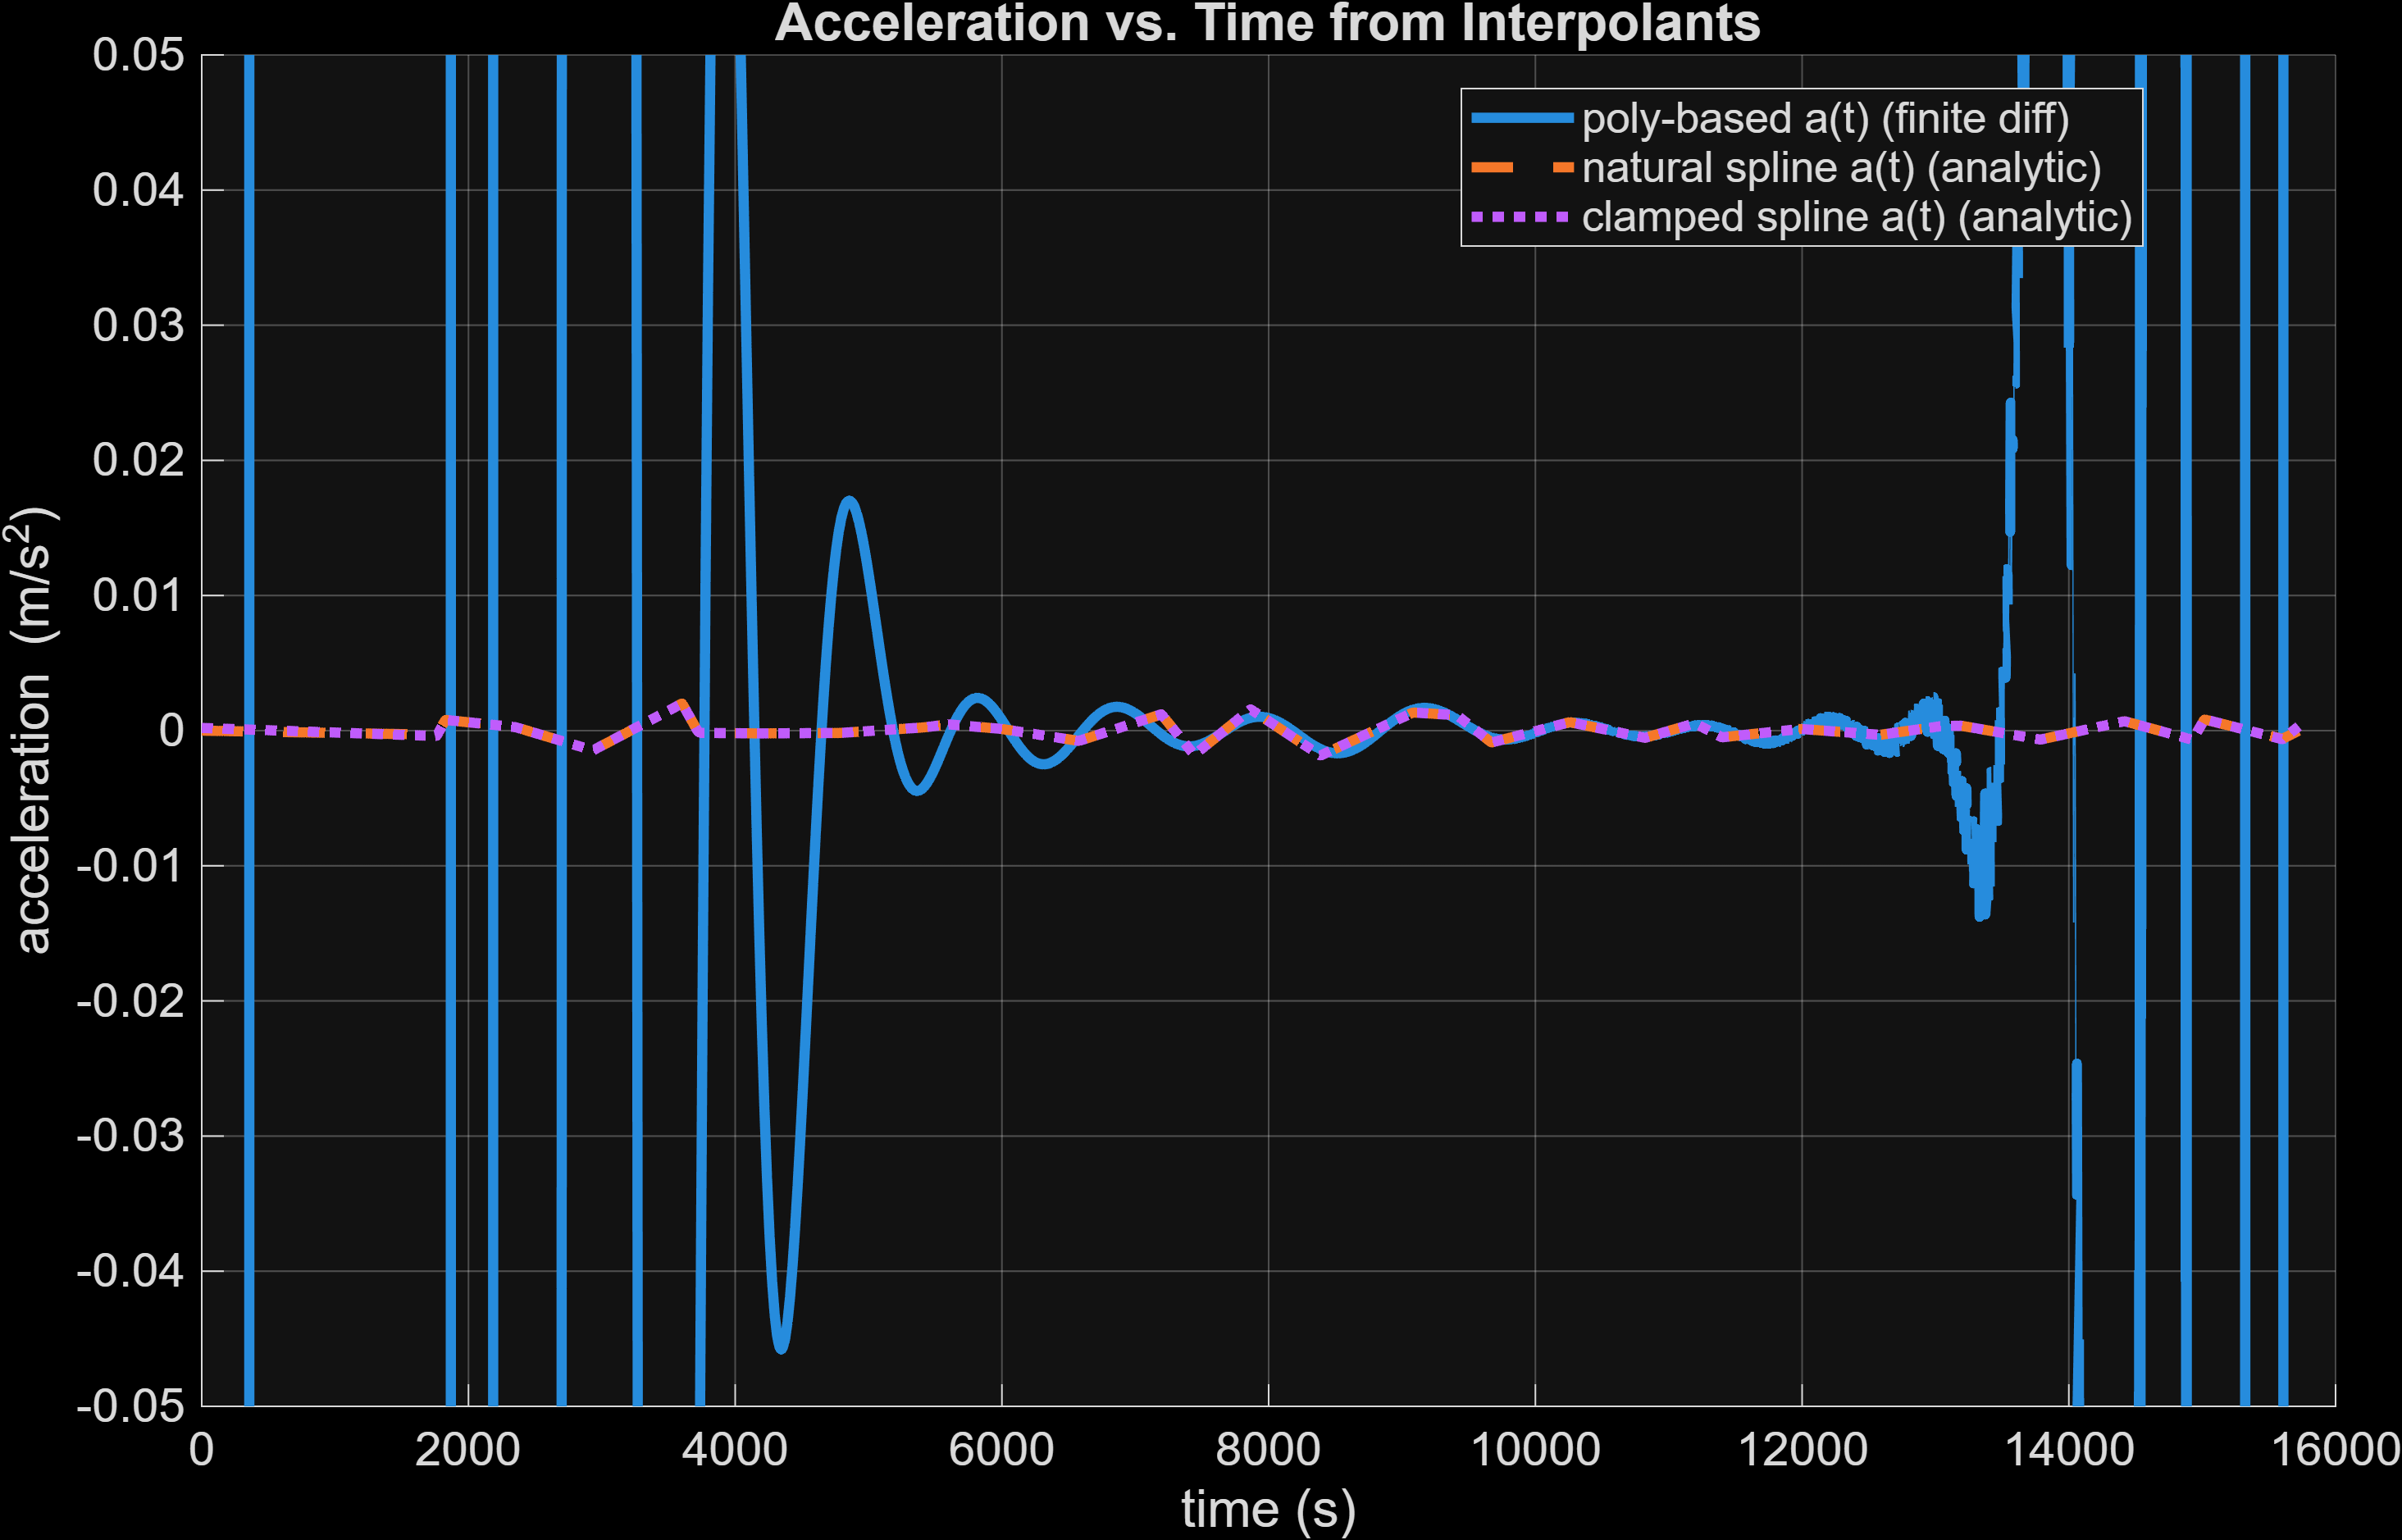
\includegraphics[width=0.85\linewidth]{VelvTime.png}
  \caption{Velocity versus time obtained from the polynomial and spline
  interpolations.}
  \label{fig:velocity}
\end{figure}

\subsection{Acceleration Profiles}

Figure~\ref{fig:acceleration} displays acceleration versus time for each
interpolant. The polynomial acceleration is computed using
finite-difference differentiation of the polynomial-derived velocities,
while spline accelerations are obtained analytically from the second
derivatives of the cubic splines.

The natural spline's acceleration curve remains near zero at both
endpoints, reflecting its enforced boundary conditions
$S''(t_0) = S''(t_n) = 0$. While mathematically smooth, this behavior
does not accurately represent the physical start of the race, where
substantial positive acceleration is expected as the runner departs from
rest, nor any late-race changes in effort.

The polynomial interpolation predicts a large positive acceleration at
the beginning of the race followed by a decreasing trend and subsequent
oscillations later in the race. Although the large initial acceleration
is physically reasonable, the oscillatory swings thereafter are not
supported by observable pace changes in the data.

The clamped spline strikes a balance between these two extremes. By
enforcing physically meaningful endpoint velocity conditions rather than
zero-curvature constraints, the clamped model allows nonzero
accelerations near the boundaries while maintaining the smooth interior
behavior of cubic splines. This produces a more realistic acceleration
profile throughout the race.

\begin{figure}[H]
  \centering
  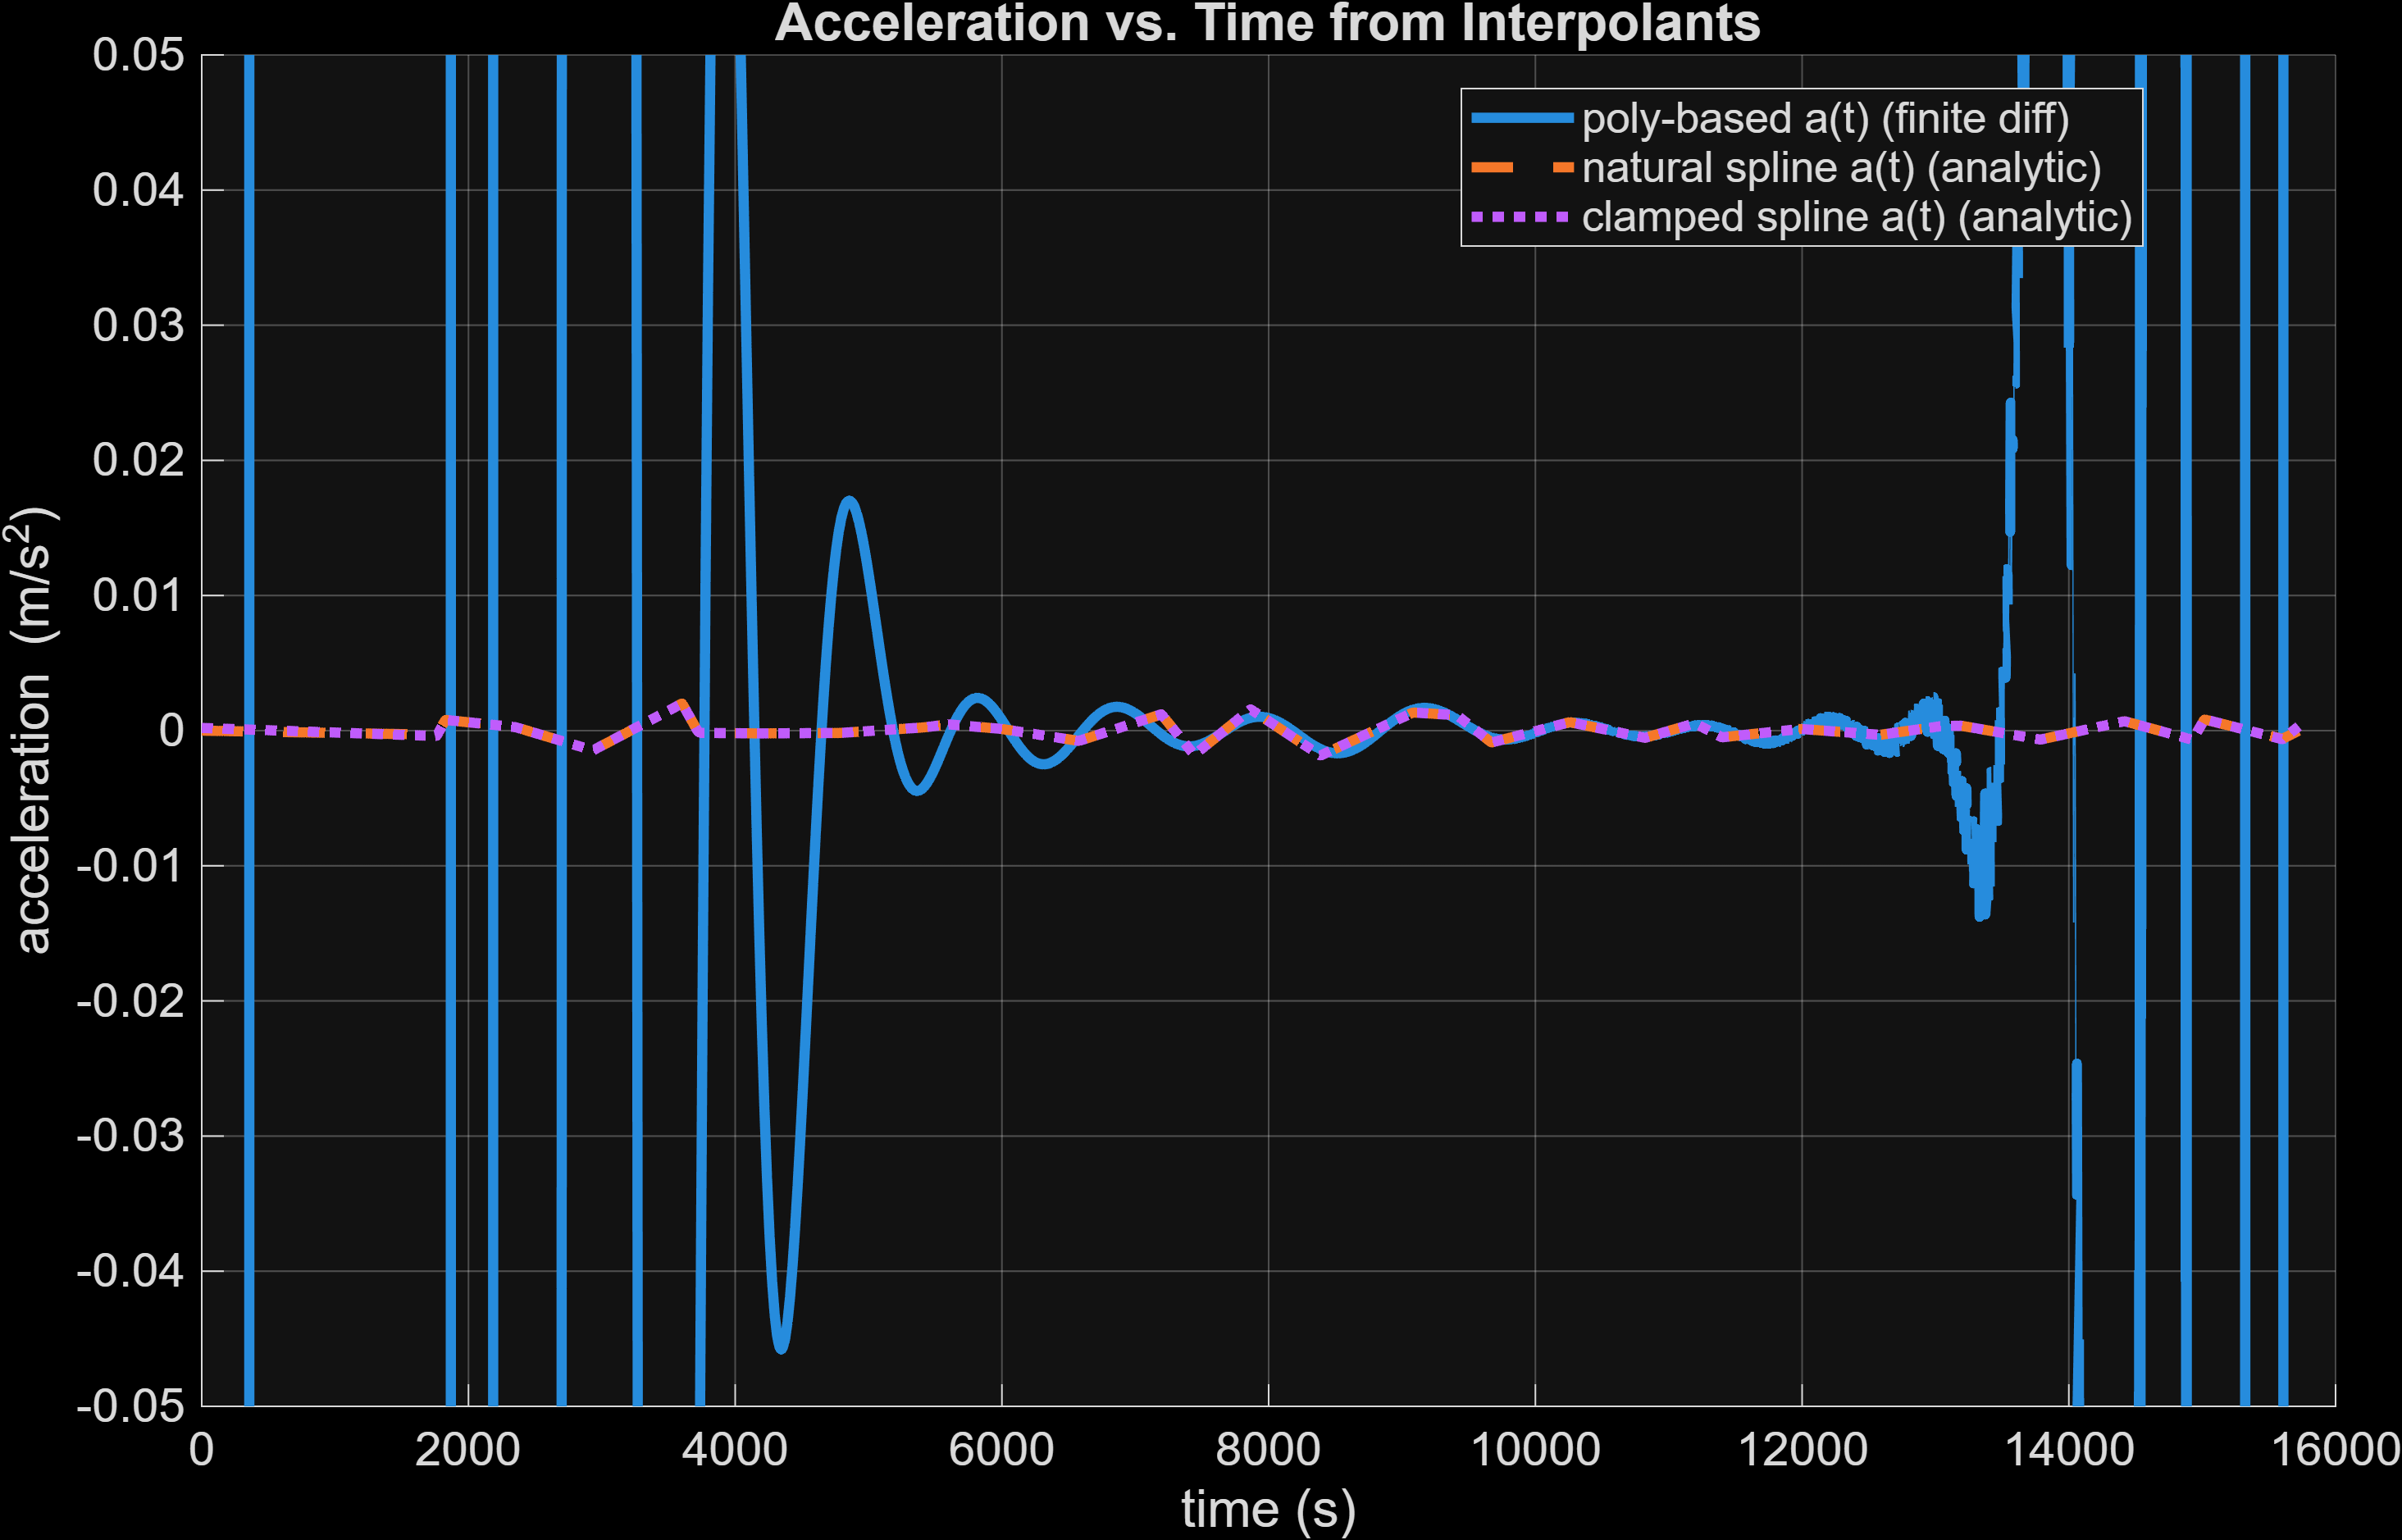
\includegraphics[width=0.85\linewidth]{AccelvTime.png}
  \caption{Acceleration versus time from each interpolation method.}
  \label{fig:acceleration}
\end{figure}

\section{Discussion}

The comparative analysis reveals distinct strengths and limitations
across the interpolation methods examined. The Newton polynomial
effectively captures sharp changes near the start of the race, including
large initial acceleration and a velocity curve beginning near zero.
However, its susceptibility to boundary oscillations generates less
realistic behavior later in the race, particularly the artificial
velocity decline near the finish seen in Figure~\ref{fig:velocity} and
the oscillatory accelerations in Figure~\ref{fig:acceleration}.

The natural cubic spline provides the smoothest overall curves but
exhibits artificially constrained endpoint behavior due to the imposed
conditions $S''(t_0) = S''(t_n) = 0$. These constraints suppress
acceleration at both the start and finish of the race, producing a
nonzero starting velocity and nearly zero terminal acceleration. While
mathematically attractive, these features conflict with the physical
dynamics of distance running, specifically the acceleration from rest at
the race start and the adjustments often observed near the finish.

The clamped cubic spline offers the most physically plausible model
across all stages of the race. By prescribing realistic endpoint
velocities instead of zero curvature conditions, the clamped spline
preserves the desirable smoothness of cubic splines while allowing
accurate representation of early acceleration and late-race surging
behavior. Its velocity and acceleration profiles align more consistently
with observed race dynamics than either the natural spline or the
polynomial interpolant.

Overall, while all methods reconstruct the position data accurately, the
differentiation process magnifies modeling assumptions. The results
demonstrate that careful selection of spline boundary conditions is
essential when derivative quantities such as velocity and acceleration
are of primary interest. Among the interpolants tested, the clamped
cubic spline provides the most balanced and physically realistic
representation of the runner's pacing profile.

\section{Conclusion and Future Work}

This project demonstrates that polynomial and spline interpolations are
useful tools for modeling a distance runner's race based on discrete
split data. Among the methods tested, the clamped cubic spline
interpolation produces the most realistic pacing curves over the full
marathon distance. High-degree polynomials perform well in capturing
short-term trends but can oscillate and generate unrealistic derivatives
towards the middle and end of the race, while natural splines can impose
endpoint behavior that is overly restrictive from a physical standpoint.

Future work could extend the current model by incorporating additional
race information, such as elevation changes or weather conditions, or by
combining interpolation with numerical integration methods introduced
later in the course. Analyzing multiple runners across different
demographics could also yield insight into how factors such as age,
gender, and racing experience influence long-distance pacing strategies.

\newpage
\begin{thebibliography}{9}

\bibitem{Dash}
S.~Dash.
\newblock Win Your Race Goal: A Generalized Approach to Prediction of Running
Performance.
\newblock \emph{Sports Medicine International Open}, 8, 2024.

\bibitem{MillettMelanson}
M.~Millett and T.~Melanson.
\newblock Predicting Running Times from Race History.

\bibitem{Sauer}
T.~Sauer.
\newblock \emph{Numerical Analysis}, 3rd ed.
\newblock Pearson, 2019.

\bibitem{CourseNotes}
Course notes and lecture slides from MTH/CSC 4150, Fall 2025.

\bibitem{NYRR}
New York Road Runners.
\newblock 2025 TCS New York City Marathon: Finishers results.
\newblock Available at \url{https://results.nyrr.org}.

\end{thebibliography}

\end{document}
